\pgfplotstablegetelem{\thepart}{[index]\columnIndex}\of{\cronograma}
\part{\pgfplotsretval}
\label{part:\thepart}
\frame{\partpage}


\begin{frame}[t]{Programação Orientada a Objetos (POO)}
	\fontsize{14pt}{15.2}\selectfont{
		Tradicionalmente a programação de sistemas considera os dados separados das funções. 

	}\par
	\vspace{1em}
	
	\fontsize{14pt}{15}\selectfont{
		\begin{itemize}%[<+->]  
			\item Os dados são	estruturados de modo a facilitar a sua manipulação pelas funções, mas as funções estão livres para usar os dados como quiserem. 
			
			\item Os aspectos segurança e integridade dos dados ficam de certa forma vulneráveis. 
			
			\item A programação tradicional de sistemas tem o seu mais forte e bem-sucedido modelo na \textbf{programação estruturada}.
			
		\end{itemize}
	}\par
	\vspace{1em}
	
\end{frame}



\begin{frame}[t]{Programação Orientada a Objetos (POO)}
	\fontsize{14pt}{15.2}\selectfont{
		Por outro lado, na programação orientada a objetos (POO), os dados específicos do objeto são estruturados junto com as funções que operam sobre esses dados. 
		
	}\par
	\vspace{1em}
	
	\fontsize{13pt}{15}\selectfont{
		\begin{itemize}%[<+->]  
			\item Linguagem como Python adota esse paradigma, onde os objetos são instâncias de classes, constituídas por variáveis (atributos) e métodos (funções) que operam sobre esses dados. 
			
			\item A POO busca robustez, adaptabilidade e reusabilidade, e seus princípios incluem modularidade, abstração e encapsulamento. 
			
			\item No desenvolvimento de software, o projeto, a implementação e os testes são etapas essenciais, e a definição clara das classes e suas responsabilidades é fundamental para o sucesso do sistema.
			
		\end{itemize}
	}\par
	\vspace{1em}
	
\end{frame}




\begin{frame}[t]{Programação Orientada a Objetos (POO)}
	
	\vspace{1em}
	\fontsize{14pt}{15}\selectfont{
		
		Na \acrfull{poo}, os dados específicos do objeto são estruturados juntamente com as funções que são permitidas sobre esses dados. Essa forma de programar é vista na linguagem Java.
		
	}\par
	\vspace{1em}
	
	
\end{frame}


\begin{frame}[t]{Programação Orientada a Objetos (POO)}
	
	\fontsize{14pt}{15}\selectfont{
		
		Os principais elementos da \acrshort{poo} são os objetos. Dizemos que um objeto é uma instância de uma classe. Uma \textbf{Classe} é constituída por variáveis (membros de dados) e métodos ou funções (membros da função).
		
	}\par
	\vspace{2em}
	
	\fontsize{14pt}{25}\selectfont{
		\begin{itemize}%[<+->]  
			\item A Classe é o modelo. Um objeto é um elemento deste modelo.
			
			\item As variáveis de uma Classe são também chamadas de \textbf{Atributos}.
			
			\item As funções de uma Classe são também chamadas de \textbf{Métodos}.
			
		\end{itemize}
	}\par
	\vspace{1em}
	
	
\end{frame}




\begin{frame}[t]{Objetivos da POO}
	
	\fontsize{14pt}{15}\selectfont{
		
		
	}\par
	\vspace{2em}
	
	\fontsize{14pt}{25}\selectfont{
		\begin{itemize}%[<+->]  
			\item Robustez – o programa não pode cair frente a dados inesperados.
			\item Adaptabilidade – rodar facilmente em diferentes ambientes.
			\item Reusabilidade – usar os elementos já construídos em outros sistemas.
			
		\end{itemize}
	}\par
	\vspace{1em}
	
	
\end{frame}



\begin{frame}[t]{Princípios da POO}
	
	\fontsize{14pt}{15}\selectfont{
		
		
	}\par
	\vspace{1em}
	
	\fontsize{14pt}{25}\selectfont{
		\begin{itemize}%[<+->]  
			\item Modularidade – dividir o sistema em pequenas partes bem definidas.
			
			\item Abstração – identificar as partes fundamentais (tipos de dados e operações), definindo o que cada operação faz e não necessariamente como é feito.
			
			\item Encapsulamento – a interface para uso de cada componente deve estar bastante clara para todos que usam esse componente. Detalhes internos de implementação não interessam.
			
		\end{itemize}
	}\par
	\vspace{1em}
	
	
\end{frame}




\begin{frame}[t]{O desenvolvimento de software}
	
	%	\fontsize{14pt}{15}\selectfont{
		%		
		%		Não há uma regra, método ou processo que oriente o desenvolvimento de bons programas e sistemas de	computador. 
		%		
		%	}\par
	\vspace{1em}
	
	\fontsize{12pt}{15}\selectfont{
		\begin{itemize}%[<+->]  
			\item Há apenas diretrizes gerais que quando usadas levam em geral a um bom resultado. 
			
			\item O desenvolvimento certamente é influenciado pelo ambiente computacional no qual será desenvolvido. 
			
			\item A	linguagem de programação e o ambiente ou plataforma na qual será desenvolvido o sistema podem decidir o	modo, a estratégia e os passos que serão usados.
			
		\end{itemize}
	}\par
	\vspace{1em}
	
	
\end{frame}



\begin{frame}[t]{O desenvolvimento de software}
	
	\fontsize{14pt}{15}\selectfont{
		
		Podemos dividir o desenvolvimento de software em 3 etapas, independente da linguagem, sistema operacional ou plataforma de desenvolvimento que será usada.
		
	}\par
	\vspace{1em}
	
	\fontsize{12pt}{15}\selectfont{
		\begin{itemize}%[<+->]  
			\item O projeto.
			
			\item A implementação.
			
			\item Os testes e depuração.
			
		\end{itemize}
	}\par
	\vspace{1em}
	
	
\end{frame}




\begin{frame}[t]{O desenvolvimento de software}
	
	\fontsize{14pt}{15}\selectfont{
		
		O projeto é a parte mais importante. Nele são definidas as classes e a relação entre elas. Os princípios que devem orientar a definição das classes são:
		
	}\par
	\vspace{1em}
	
	\fontsize{12pt}{15}\selectfont{
		\begin{itemize}%[<+->]  
			\item \textbf{Responsabilidade de cada uma delas} – quais problemas elas resolve.
			
			\item \textbf{Independência entre elas} – se uma precisa da outra e vice-versa.
			
			\item \textbf{Comportamento} – quais as entradas (parâmetros) e saídas (resultados) das classes.
			
		\end{itemize}
	}\par
	\vspace{1em}
	
	\url{https://docs.python.org/pt-br/3/tutorial/classes.html}
	
\end{frame}





\begin{frame}[t]{Resumo sobre Programação Orientada a Objetos}
	
	\fontsize{10pt}{15}\selectfont{
		
		Os princípios básicos da \acrshort{poo} são descritos a seguir.
		
	}\par
	\vspace{0.5em}
	
	\fontsize{10pt}{13}\selectfont{
		\begin{itemize}%[<+->]  
			\item \textbf{Classe}: Representação de um conjunto de objetos com características afins. Definição do comportamento dos objetos (métodos) e seus atributos. 
			
			\item \textbf{Objeto}: Uma instância de uma classe. Armazena estados por meio de atributos e reação a mensagens enviadas por outros objetos.
			
			\item \textbf{Abstração}: Oculta detalhes que não são necessários no contexto.
			
			\item \textbf{Herança}: Mecanismo pela qual uma classe (sub-classe) pode estender outra classe (super-classe), estendendo seus comportamentos e atributos.
			
			\item \textbf{Polimorfismo}: Princípio pelo qual as instâncias de duas classes ou mais classes derivadas de uma mesma super-classe podem invocar métodos com a mesma assinatura, mas com comportamentos distintos. 
			
			\item \textbf{Encapsulamento}: Proibição do acesso direto ao estado de um objeto, disponibilizando apenas métodos que alterem esses estados na interface pública. 
			
		\end{itemize}
	}\par
	\vspace{1em}
	
\end{frame}




\begin{frame}[t]{Um exemplo de programação orientada a objeto com Python}
	
	\fontsize{14pt}{15}\selectfont{
		
		Vamos desenvolver um sistema que possui produtos. O objeto em questão é o produto. Assim, vamos criar a classe Produto, que tornará possível construir ou criar elementos ou objetos desta classe.
		
	}\par
	\vspace{1em}
	
	A sintaxe básica para criação de uma classe é´:
	
	\vspace{1em}
	\begin{beamercolorbox}[wd=\textwidth]{warning}
		class {NomeDaClasse}: \\
		\hspace{1em}{Instruções}
	\end{beamercolorbox}
	
	\vspace{1em}
	\fontsize{12pt}{15}\selectfont{
		\begin{itemize}%[<+->]  
			\item \textbf{classe} - Produto.
			
			\item \textbf{atributos} - nome, codigo, preco, quantidade.
			
			\item \textbf{métodos} - obtem\_nome, obtem\_codigo, obtem\_preco, altera\_preco, altera\_quantidade.
			
		\end{itemize}
	}\par
	\vspace{1em}
	
	
\end{frame}


\begin{frame}[t]{Requisitos da classe Produto}
	
	\fontsize{14pt}{15}\selectfont{
		
		Vamos listar abaixo:
		
	}\par
	\vspace{1em}
	
	
	\fontsize{12pt}{15}\selectfont{
		\begin{itemize}%[<+->]  
			\item Deve ser possível recuperar o nome, código e preço do produto.
			
			\item Devolve True se novo preço for maior que o atual preço.
			
			\item Devolve False se a quantidade de produtos requerida não está disponível.
			
		\end{itemize}
	}\par
	\vspace{1em}
	
	
\end{frame}



\begin{frame}[t]{Atenção}
	
%	\vspace{1em}
%	\fontsize{14pt}{19}\selectfont{
%		Escreva utilizando algoritmo.
%	}\par
%	
%	\vspace{1em}
%	
%	\centering
%	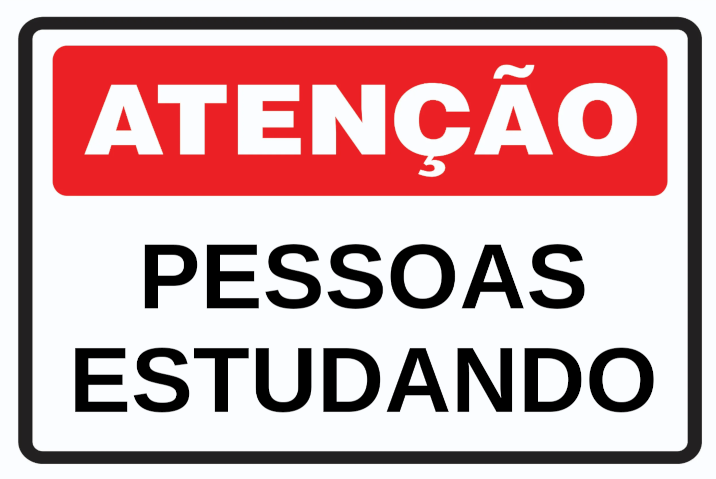
\includegraphics[scale=0.4]{imagens/fig-atencao-pessoas-estudando.png}
	
%	\parbox{1\linewidth}{ 
	\centering
	\begin{tikzpicture}
%		\node at (0,0){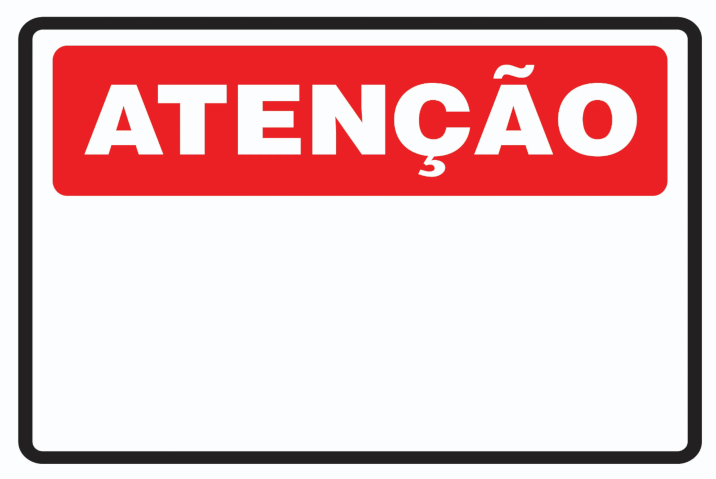
\includegraphics[width=0.7\textwidth]{imagens/fig-atencao-fundo-branco.png}
		\node (image) 
		{
			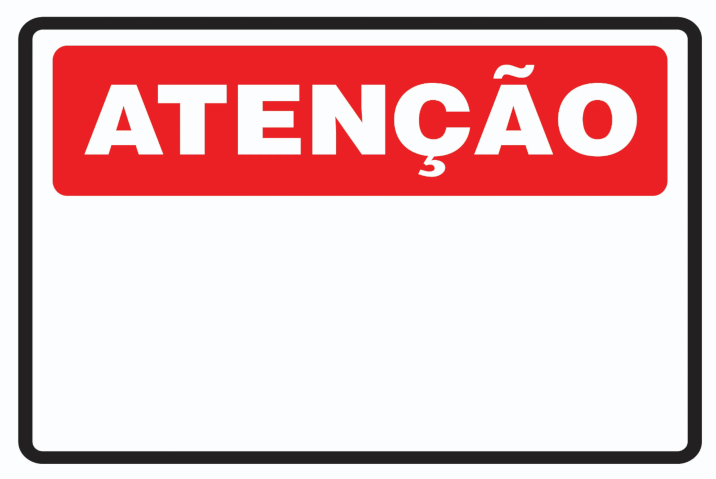
\includegraphics[width=0.7\textwidth]{imagens/fig-atencao-fundo-branco.png}
		};
		\node
		[
		%		fill=teal,
		overlay,
		align=center,
		text=black,
		font={\fontsize{34pt}{19}\bfseries}
		] at (0,-1) (image.center) {Respirem fundo\\ que vamos...};
	\end{tikzpicture}
%	}

	
\end{frame}



\begin{frame}[t]{Exemplos de criação de classe}	
	
	\lstinputlisting[style=CBruno,caption=Código da classe Produto]{outros/codigos/python/codigo_003_classe_produto.py}
	
	\vspace{1em}
	
	
\end{frame}


\begin{frame}[t]{Exemplos de criação de classe}	
	
	
	\fontsize{14pt}{15}\selectfont{
		
		Se o código abaixo for colocado junto com o arquivo da classe Produto, é posssível "testar" o código no mesmo arquivo. É desaconselhável fazer.
		
	}\par
	\vspace{1em}
	
	\fontsize{14pt}{25}\selectfont{
		\begin{beamercolorbox}[wd=\textwidth]{warning}
			if \_\_name\_\_ == "\_\_main\_\_":\\
			\hspace{1em}p1 = Produto("Laranja", 1, 1.56, 10)\\
			\hspace{1em}print("Oferta do dia:", p1.obtem\_nome())\\
			\hspace{1em}if p1.altera\_preco(40.00): print("Preco alterado hoje")\\
			\hspace{1em}else: print("Atencao - baixou o preco")
		\end{beamercolorbox}
		
	}\par
	\vspace{1em}
	
\end{frame}




\begin{frame}[t]{Pytest}
	
	\vspace{-2em}
	\lstinputlisting[style=CBruno,caption=Cobertura de testes da classe Produto]{outros/codigos/python/test_codigo_003_classe_produto.py}
	
	
	
\end{frame}



\begin{frame}[t]{Pytest}
	
	
	\vspace{1em}
	\centering
	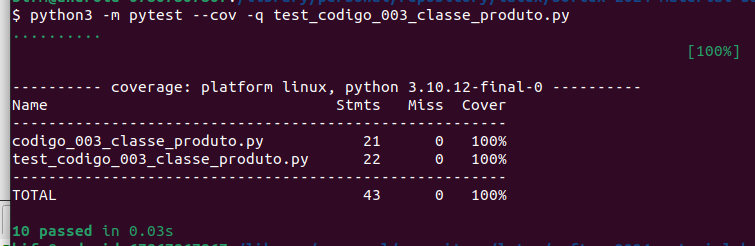
\includegraphics[scale=0.5]{imagens/fig-result-test-class-produto.png}
	
\end{frame}




\begin{frame}[t]{classe Produto}
	
	\fontsize{14pt}{15}\selectfont{
		
		O nome \textbf{self} refere-se ao particular objeto sendo criado. Note que o primeiro parâmetro é sempre self na definição. No uso ou na chamada do método esse primeiro parâmetro não existe.
		
	}\par
	\vspace{1em}
	
	
	\fontsize{12pt}{15}\selectfont{
		\begin{itemize}%[<+->] 
			
			\item No exemplo anterior incluímos além da definição da classe, alguns comandos de teste dos métodos da mesma. Assim o módulo (arquivo onde está armazenada a classe) poderia chamar-se Produto.py.
			
			\item O comando if \textbf{\_\_name\_\_} == “\textbf{\_\_main\_\_}” usado antes dos testes anteriormente, determina que os comandos abaixo somente serão executados quando a classe estiver sendo testada, isto é, quando for solicitada a execução do módulo Produto.py
			
		\end{itemize}
	}\par
	\vspace{1em}
	
	
\end{frame}




\begin{frame}[t]{Uso e declaração dos métodos}
	
	\fontsize{14pt}{15}\selectfont{
		
		Quando o método é declarado sempre o primeiro parâmetro é self, quando é necessário acesso ao objeto.	Entretanto nas chamadas omite-se esse parâmetro. O correspondente ao self torna-se o prefixo da chamada.
		
	}\par
	\vspace{1em}
	
	
	Declaração:
	\vspace{1em}
	\begin{beamercolorbox}[wd=\textwidth]{warning}		
		def altera\_preco(self, novo\_preco):\\
		\hspace{1em}{Instruções}
	\end{beamercolorbox}
	
	
	Uso:
	\vspace{1em}
	\begin{beamercolorbox}[wd=\textwidth]{warning}
		p1 = Produto("Arroz", 1, 2, 5)\\
		if p1.altera\_preco(2): print('False')
	\end{beamercolorbox}
	
	
\end{frame}



\begin{frame}[t]{O método construtor}
	
	\fontsize{14pt}{15}\selectfont{
		
		\textbf{\_\_init\_\_} é um método especial dentro da classe. É construtor da classe, onde os atributos do objeto recebem seus valores iniciais. 
		
	}\par
	\vspace{1em}
	
	
	\fontsize{12pt}{15}\selectfont{
		\begin{itemize}%[<+->] 
			
			\item No caso da classe acima, os 4 atributos (variáveis) que caracterizam um produto, recebem neste método seus valores iniciais, que podem ser modificados por operações futuras deste mesmo objeto. 
			
			\item A criação de um novo produto, ou seja, a criação de uma instância do objeto produto causa a execução do método \textbf{\_\_init\_\_}. Assim, o comando abaixo, causa a execução do método \textbf{\_\_init\_\_}:
			
			
			\vspace{1em}
			\begin{beamercolorbox}[wd=\textwidth]{warning}
				p1 = Produto("Arroz", 1, 2, 5)
			\end{beamercolorbox}
			
		\end{itemize}
	}\par
	\vspace{1em}
	
\end{frame}



\begin{frame}[t]{Explorar a sintaxe das classes – o parâmetro self}
	
	\fontsize{14pt}{15}\selectfont{
		
		O parâmetro self é importante no método construtor da classe \textbf{\_\_init\_\_}, para referenciar o objeto que está sendo criado. Nos demais métodos, se usado, é simplesmente um parâmetro. Nem precisa ser o primeiro. Mesmo no \textbf{\_\_init\_\_}, o primeiro parâmetro pode ter qualquer nome. 
		
	}\par
	\vspace{1em}
	
	\fontsize{14pt}{25}\selectfont{
		\begin{beamercolorbox}[wd=\textwidth]{warning}
			class Produto:\\
			\hspace{1em}def \_\_init\_\_(outro, nome):\\
			\hspace{2em}outro.nome = nome\\
			
			
			\hspace{1em}def altera\_nome(nome, self):\\
			\hspace{2em}self.nome = nome
		\end{beamercolorbox}
		
	}\par
	\vspace{1em}
	
\end{frame}




\begin{frame}[t]{Explorar a sintaxe das classes – o parâmetro self}
	
	
	
	\fontsize{12pt}{15}\selectfont{
		\begin{itemize}%[<+->] 
			
			\item No caso da classe acima, os 4 atributos (variáveis) que caracterizam um produto, recebem neste método seus valores iniciais, que podem ser modificados por operações futuras deste mesmo objeto. 
			
			\item A criação de um novo produto, ou seja, a criação de uma instância do objeto produto causa a execução do método \textbf{\_\_init\_\_}. Assim, o comando abaixo, causa a execução do método \textbf{\_\_init\_\_}:
			
			
			\vspace{1em}
			\begin{beamercolorbox}[wd=\textwidth]{warning}
				p1 = Produto("Arroz", 1, 2, 5)
			\end{beamercolorbox}
			
		\end{itemize}
	}\par
	\vspace{1em}
	
\end{frame}



\begin{frame}[t]{Explorar a sintaxe das classes}
	
	\fontsize{14pt}{15}\selectfont{
		
		Uma classe não precisa necessariamente ter um método construtor. Podemos ter uma classe apenas com métodos, sem atributos. Nesse caso, o nome da classe é usado sem parâmetros para a chamada das funções.
		
	}\par
	\vspace{1em}
	
	\fontsize{14pt}{25}\selectfont{
		\begin{beamercolorbox}[wd=\textwidth]{warning}
			class Produto:\\		
			
			\hspace{1em}def imprime\_nome(nome):\\
			\hspace{2em}print(nome)\\
			\vspace{1em}
			Produto.imprime\_nome('Arroz')
			
		\end{beamercolorbox}
		
	}\par
	\vspace{1em}
	
\end{frame}



\begin{frame}[t]{Herança em classes}
	
	\fontsize{14pt}{15}\selectfont{
		
		Permite que uma classe seja definida com base em classe já existente. Dizemos que essa nova classe herda características da classe original. 
		
	}\par
	\vspace{1em}
	
	\fontsize{12pt}{15}\selectfont{
		\begin{itemize}%[<+->] 
			
			\item Na terminologia Python a classe original é chamada de Classe Base, Classe Mãe ou Superclasse (Base, Parent ou Super Class) enquanto que a nova é chamada de Sub Classe ou Classe Filha (Sub ou Child Class).
			
			\item A subclasse pode especializar a classe principal ou mesmo estendê-la com novos métodos e atributos.
			
		\end{itemize}
	}\par
	\vspace{1em}
	
\end{frame}





\begin{frame}[t]{Herança em classes}
	
	\fontsize{14pt}{15}\selectfont{
		
		Uma classe não precisa necessariamente ter um método construtor. Podemos ter uma classe apenas com métodos, sem atributos. Nesse caso, o nome da classe é usado sem parâmetros para a chamada das funções.
		
	}\par
	\vspace{1em}
	
	\fontsize{14pt}{25}\selectfont{
		\begin{beamercolorbox}[wd=\textwidth]{warning}
			class Produto:\\		
			
			\hspace{1em}def imprime\_nome(nome):\\
			\hspace{2em}print(nome)\\
			\vspace{1em}
			Produto.imprime\_nome('Arroz')
			
		\end{beamercolorbox}
		
	}\par
	\vspace{1em}
	
\end{frame}



\begin{frame}[t]{Herança em classe}	
	
	\lstinputlisting[style=CBruno,caption=Herança da classe Produto]{outros/codigos/python/codigo_004_classe_produto_critico.py}
	
	
	*obs: \textbf{class ProdutoCritico(Produto)} é uma classe derivada de Produto: indica que \textbf{ProdutoCritico} é uma subclasse da classe \textbf{Produto}.
	
\end{frame}

\begin{frame}[t]{Pytest}
	
	\vspace{-1em}
	\lstinputlisting[style=CBruno,caption=Cobertura de testes da classe Produto Crítico]{outros/codigos/python/test_codigo_004_classe_produto_critico.py}
	
	
\end{frame}



\begin{frame}[t]{Pytest}
	
	
	\vspace{1em}
	\centering
	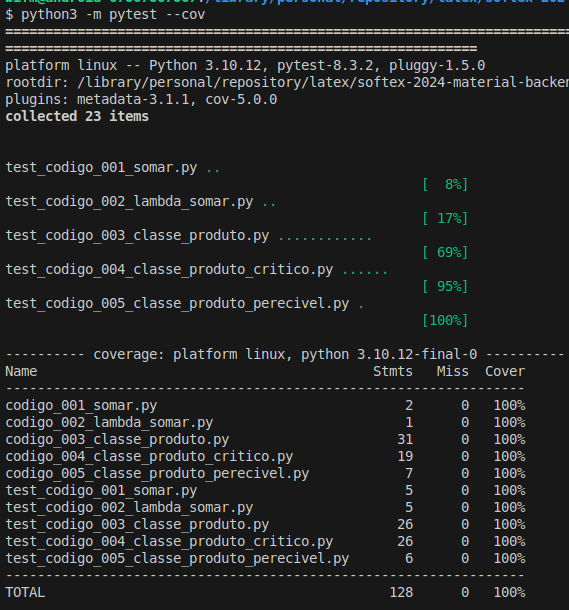
\includegraphics[scale=0.3]{imagens/fig-result-test-produto-critico.png}
	
\end{frame}





\begin{frame}[t]{Polimorfismo em classe}
	
	\fontsize{14pt}{15}\selectfont{
		
		Polimorfismo permite que objetos de diferentes classes sejam tratados como objetos de uma classe comum.
		
	}\par
	\vspace{1em}
	
	\fontsize{12pt}{15}\selectfont{
		\begin{itemize}%[<+->] 
			
			\item Polimorfismo é o princípio pelo qual duas ou mais classes derivadas de uma mesma superclasse podem invocar métodos que têm a mesma identificação, assinatura, mas comportamentos distintos, especializados para cada classe derivada, usando para tanto uma referência a um objeto do tipo da superclasse.
			
			%			\item 
			
		\end{itemize}
	}\par
	\vspace{1em}
	
\end{frame}






\begin{frame}[t]{Polimorfismo em classe}	
	
	\lstinputlisting[style=CBruno,caption=Polimorfismo de classe]{outros/codigos/python/codigo_005_classe_produto_perecivel.py}
	
	\vspace{1em}
	
	*obs: \textbf{class ProdutoPerecivel(Produto)} é uma classe derivada de Produto: indica que \textbf{ProdutoPerecivel} é uma subclasse da classe \textbf{Produto}.
	
\end{frame}

\begin{frame}[t]{Pytest}
	
	%	\vspace{-2em}
	\lstinputlisting[style=CBruno,caption=Cobertura de testes da classe Produto Perecivel]{outros/codigos/python/test_codigo_005_classe_produto_perecivel.py}
	
	
\end{frame}




\begin{frame}[t]{Pytest}
	
	\centering
	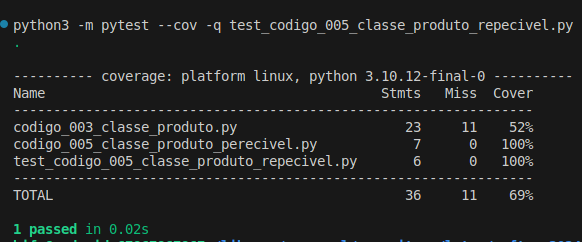
\includegraphics[scale=0.5]{imagens/fig-result-test-especifico-produto-perecivel.png}
	
\end{frame}


\begin{frame}[t]{Pytest}
	
	\centering
	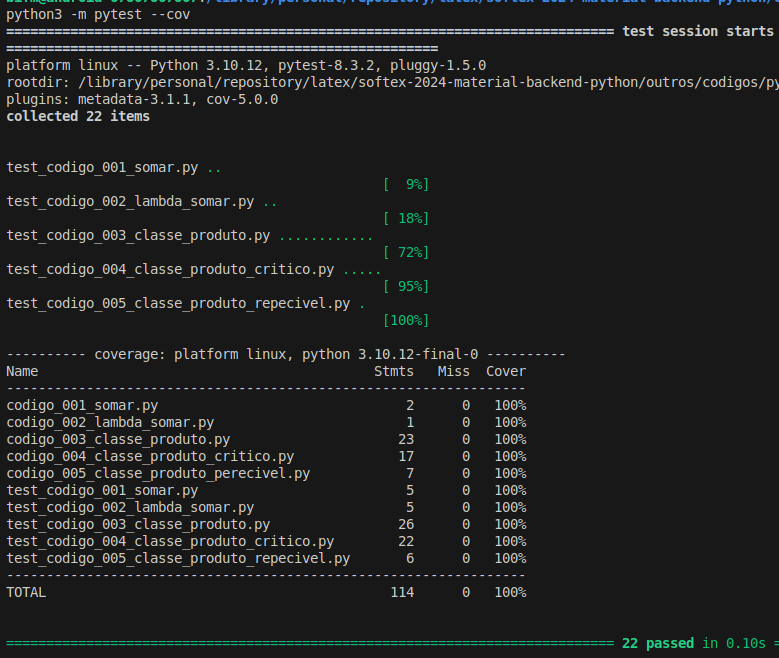
\includegraphics[scale=0.3]{imagens/fig-result-test-produto-perecivel.png}
	
\end{frame}






\begin{frame}[t]{Polimorfismo em classe}	
	
	\fontsize{14pt}{15}\selectfont{
		
		Sobreposição.
		
	}\par
	\vspace{1em}
	
	\fontsize{12pt}{15}\selectfont{
		\begin{itemize}%[<+->] 
			
%			\item Sobrecarga (Overload): é o ato de criar vários métodos diferentes com o mesmo o nome, porém com assinaturas diferentes, cada um com sua própria implementação. Python não trabalha com overload por padrão. Para alcançar é possível utilizar bibliotecas com decoratores.
			
			\item Sobreposição (Override): é sobrescrever, ou seja, definir um novo comportamento para um método que já existe. Isso acontece quando a classe em questão herda (estende) outra classe e se cria um método com a mesma assinatura da classe "pai" na classe filha.
			
		\end{itemize}
	}\par
	\vspace{1em}
	
\end{frame}



\begin{frame}[t]{Encapsulamento em classe}
	
	\fontsize{12pt}{15}\selectfont{
		
		Encapsulamento é a proteção dos atributos ou métodos de uma classe, em Python existem somente o public e o private e eles são definidos no próprio nome do atributo ou método.
		
	}\par
	
	\vspace{0.5em}
	\fontsize{8pt}{10}\selectfont{
		\begin{beamercolorbox}[wd=\textwidth]{warning}
			class Veiculo:\\
			\hspace{1em}chassi = 1 \# atributo publico\\
			\hspace{1em}\_\_motor = 2 \# atributo privado a classe Veiculo. O símbolo \_\_* define como privado.\\
			\vspace{0.5em}
			class Carro(Veiculo):\\
			\hspace{1em}\_\_placa = 3 \# atributo privado a classe Carro\\
			\vspace{0.5em}
			\hspace{1em}def \_\_init\_\_(self):\\
			\hspace{2em}print(self.chassi)\\
			\hspace{2em}print(self.\_\_placa)\\
			\vspace{0.5em}
			veiculo = Veiculo()\\
			print(veiculo.chassi) \# imprime 1\\
			\vspace{0.5em}
			carro = Carro() \# Erro\\
			\# print(carro.\_\_motor) \# Erro, pois \_\_motor é privado a classe Veiculo.\\
			\# print(carro.\_\_placa) \# Erro, \_\_placa é um atributo privado, somente chamado pela classe Carro.\\
		\end{beamercolorbox}
		
	}\par
	\vspace{1em}
	
	
\end{frame}






\begin{frame}[t]{Encapsulamento em classe}
	
	\begin{block}{Exemplo anteior}		
		class Veiculo:\\
		\hspace{1em}chassi = 1 \# atributo publico\\
		\hspace{1em}\_\_motor = 2 \# atributo privado a classe Veiculo. O símbolo \_\_* define como privado.\\
		\vspace{0.5em}
		class Carro(Veiculo):\\
		\hspace{1em}\_\_placa = 3 \# atributo privado a classe Carro\\
		\vspace{0.5em}
		\hspace{1em}def \_\_init\_\_(self):\\
		\hspace{2em}print(self.chassi)\\
		\hspace{2em}print(self.\_\_placa)\\
		\vspace{0.5em}
		veiculo = Veiculo()\\
		print(veiculo.chassi) \# imprime 1\\
		\vspace{0.5em}
		carro = Carro() \# Erro\\
		\# print(carro.\_\_motor) \# Erro, pois \_\_motor é privado a classe Veiculo.\\
		\# print(carro.\_\_placa) \# Erro, \_\_placa é um atributo privado, somente chamado pela classe Carro.\\
	\end{block}
	
	
\end{frame}




\begin{frame}[t]{Tratamento de exceções}
	
	\fontsize{13pt}{15}\selectfont{
		
		O tratamento de exceção, na ciência da computação, é o mecanismo responsável pelo tratamento da ocorrência de condições que alteram o fluxo normal da execução de programas de computadores. \\Para condições consideradas parte do fluxo normal de execução, ver os conceitos de sinal e evento.
		
	}\par
	
	\vspace{2em}
	Saiba mais em
	\url{https://docs.pytest.org/en/stable/how-to/assert.html}
	
\end{frame}







\begin{frame}[t]{Tratamento de exceções}
	
	\vspace{1em}
	
	\fontsize{13pt}{15}\selectfont{
			A sintaxe básica é:		
	}\par
	
	\vspace{1em}
	\begin{beamercolorbox}[wd=\textwidth]{warning}
		try: \\
		\hspace{1em}{Instruções} \# o código da funcionalidade.\\
		...\\
		except <ExceptType>:\\
		\hspace{1em}{Instruções} \# o código para tratamento da exceção.\\
		...\\
		finally: \# Caso o fluxo não seja interrompido, sempre é executado o finally.\\
		\hspace{1em}{Instruções}
	\end{beamercolorbox}
		
	
	\vspace{2em}
	\url{https://docs.python.org/pt-br/3/tutorial/errors.html}
	
\end{frame}














\begin{frame}[t]{Tratamento de exceções}	
	
	\lstinputlisting[style=CBruno,caption=Tratamento de exceções]{outros/codigos/python/codigo_006_classe_veiculo_com_exception.py}
	
	
\end{frame}





\begin{frame}[t]{Pytest}
	
	%	\vspace{-2em}
	\lstinputlisting[style=CBruno,caption=Cobertura de testes da classe Veiculo]{outros/codigos/python/test_codigo_006_classe_veiculo_com_exception.py}
	
	
\end{frame}


